\chapter{Existující přístupy}

\begin{table*}[t]\footnotesize
\begin{center}
\begin{tabular}{| l || c || c | c || c | c || c | c | c |}
\hline
Metoda DDA & vážná hra & explicitní & implicitní & statická & dynamická & NPC & svět & úkoly \\
\hline
\hline
Částečně pozorovatelné markovské rozhodovací procesy &  & & & & & & \\ \hline
Producent – konzument & & & & & & & \\ \hline
Case-base reasoning & & & & & & & \\ \hline
Fuzzy pravidla & & & & & & & \\ \hline
Evoluční algoritmus & & & & & & & \\ \hline
Mravenčí feromony & & & & & & & \\ \hline
Částečně uspořádaná množina – Mistr& \checkmark & & & & & & \\ \hline
Dynamická úroveň & & & & & & & \\ \hline
Monte-Carlo prohledávání stromu & & & & & & & \\ \hline
\end{tabular}
\end{center}
\vspace*{0mm}
\caption{{\label{tab:tab1}}Příklad tabulky. Další popis i upřesnění
  parametrů může následovat v této legendě.}
\vspace*{0mm}
\label{shadowtable}
\end{table*}


\section{Ne z teorie her}

\subsection{Částečně pozorovatelné markovské rozhodovací procesy}

Částečně pozorovatelné markovské rozhodovací procesy (POMDP) byly úspěšně použity pro regeneraci rukou lidí po mrtvici \cite{9Pomdp} a u počítačového asistenta při mytí rukou člověkem trpícím demencí.

V obou případech byla osoba se systémem modelováno pomocí POMDP, které jsou schopné pracovat se sekvenčními dynamickými systémy, ve kterých jsou některé stavy preferované před jinými a ne vše související s procesem je plně pozorovatelné. V těchto případech nelze přímo pozorovat aktuální schopnosti uživatele.

V každém kroku je uložen belief state (pravděpodobnostní distribuce nad všemi stavy). Policy (politika) říká, kterou akci v daném kroku vybrat na základě aktuální belief state, které se na základě vybrané akce a nového pozorování aktualizuje.

\subsubsection{Influence diagramy}

Obecná POMDP mohou být řešena více exaktními způsoby, ale nejsou řešitelná s dostatečně krátkou odezvou pro naše využití. POMDP pro popsané úlohy může být redukováno na influence diagramy, které jsou snáze řešitelné.
 
Obecný influence diagram pro adaptivní systém si lze prohlédnout na Obr.~\ref{fig:ch3pomdp}. Apostrofované proměnné představují odpovídající neapostrofované proměnné v následujícím stavu. Např. hodnota napětí v následujícím stavu závisí pouze na hodnotách schopnosti a provedené akce z předchozího stavu.

\begin{figure}
  \centering
  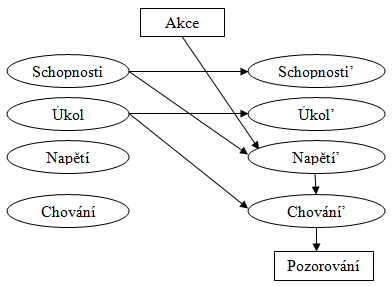
\includegraphics[width=0.5\textwidth]{ch3pomdp}
	\caption{Influence diagram pro adaptivní systémy}
	\label{fig:ch3pomdp}
\end{figure}

V každém kroku se provede právě jedna akce. Stav je popsán proměnnými 4 kategorií. Proměnná schopnosti(ability) je odhadem aktuálních schopností uživatele. Proměnná úkol(task) popisuje aktuálně prováděný úkol osobou. Proměnná napětí(stretch) znázorňuje náročnost aplikace vzhledem k aktuálnímu uživateli. Popisuje rozdíl úrovně obtížnosti zvolené akce a úrovně schopností jedince. Ideálně jsou úrovně shodné, napětí je nulové. Pokud je napětí vysoké, úkol je příliš obtížný. Jestliže je napětí záporné, úkol je příliš snadný. Proměnná chování(behavior) je přímo pozorovatelná. U pomocníka při mytí rukou je jím pozice rukou (ve vodě, na kohoutku atd.) a stav puštění vody.

\subsubsection{Příklad popisu stavu hry}

Pro lepší pochopení skupin proměnných a jejich významu uvedu příklady proměnných uvedených v článku \cite{9Pomdp}, rehabilitace po mozkové mrtvici.

Schopností je rychlost učení, jak rychle se každý uzdravuje. Úkol popisuje vektor n(r), kde pro jednotlivé hodnoty odporu ovladače je uložena maximální vzdálenost, kterou je osoba schopna dosáhnout. Napětí zde má zachován svůj význam z obecného popisu. Chování je zde nahrazeno celkovou únavou, která souvisí s následujícími pozorovanými veličinami. TTT, čas potřebný k dosáhnutí na cíl, CTRL, reprezentuje, jestli bylo cvičení vykonáno s pomocí kontroly, COMP, jestli si osoba snažila pomáhat vrchní polovinou těla místo využívání pouze její paže.

Konkrétní influence diagram můžeme vyřešit např. pomocí algoritmu PERSEUS, který najde v dostatečně krátkém čase přibližné řešení. Na základě pozorování a provedených akcí dokáže odhadnout schopnosti uživatele a vzhledem k tomu připravit odpovídající následující úlohu.

\subsection{Producent – konzument}

V mnohých hrách můžeme pozorovat vztah producent – konzument mezi světem a hráčem. Jestliže hráč získá ze světa moc prostředků, hra přestává být výzvou a naopak. Má-li hráč málo prostředku (např. munice, zdraví), může být frustrován kvůli vysoké obtížnosti.
Robin Hunicke popsala systém The Hamlet integrovaný do Half-Life SDK\cite{20Hun}, který vyvažuje obtížnost hry právě pomocí výměny zdrojů mezi světem a hráčem. Half-Life patří mezi klasické zástupce first-person shooter (FPS, „střílečky“).

\subsubsection{Použitá metrika}

Hunicke používá metriku pravděpodobnost smrti hráče. Ze série měření určí pravděpodobnostní distribuci poškození udělené hráči protivníkem během boje. Předpokládá Gaussovskou distribuci :

\begin{equation}
	   p(x)=\frac{1}{\sigma\sqrt{2\pi}}\mathrm{e}^{\frac{-(x-\mu)^2/2}{\sigma^2}}
\end{equation}

Pomocí určitého integrálu F(d) můžeme spočítat pravděpodobnost utrpění poškození menší, nebo rovnu d, kterou lze využít pro určení pravděpodobnosti přežití, jestliže má hráč aktuální zdraví rovné hodnotě d.

\begin{equation}
	   F(x) = \int_d^\infty p(x)\,\mathrm{d}x
\end{equation}

Dosazením za p(x) získáváme rovnici \ref{eq:integraldamage}.

\begin{equation} \label{eq:integraldamage}
	   F(x) = \frac{1}{\sigma\sqrt{2\pi}}\int_d^\infty \mathrm{e}^{\frac{-(x-\mu)^2/2}{\sigma^2}}\,\mathrm{d}x
\end{equation}

Tento integrál lze aproximovat funkcí erf z knihovny C++. V následujícím vzorci h odpovídá aktuálnímu zdraví hráče, $\mu, \sigma$ pro střední hodnotu a standardní odchylku poškození od aktuálního oponenta v nějakém čase t v budoucnu.

\begin{equation}
	   F(d_t) = 1-\frac{1}{2}(1+erf(\frac{h-\mu t}{\sigma\sqrt{2t}}))
\end{equation}

Během souboje se zaznamenává poškození d, které každý z protivníků udělí hráči. Na základě těchto hodnot a vzorců výše lze přibližně spočítat pravděpodobnost smrti hráče.

\subsubsection{Vyvažující strategie}

Systém Hamlet mění obtížnost na základě poptávky a nabídky. Na straně nabídky může systém zasáhnout umisťováním předmětů v herním prostředí (lékárničky, munice, zbraně). Dále může přizpůsobovat účinnost a přesnost hráčových zbraních, projev brnění apod.

Na straně poptávky manipulovat s nepřáteli (změnou jejich třídy, množství, počtu jejich životů, určením místa jejich objevení se na mapě). Stejně jako u hráče lze přizpůsobit sílu a přesnost jejich zbraní.

Autoři se snaží držet hráče v tzv. „komfortní zóně“, kdy se hráč cítí relativně v bezpečí. Jestliže se v průběhu boje zvedne pravděpodobnost úmrtí nad 40\%, Hamlet začne zasahovat do hry výše uvedenými způsoby.

Cílem této politiky je udržet zdraví hráče na střední hodnotě 60 se standardní odchylkou 15 bodů. Hamlet je navržen tak, aby pomáhal hráčům, kteří mají problémy, ale na druhou stranu, aby je neprotahoval za každou cenu skrz herní úrovně.

\subsection{Case-base reasoning}

Další možností pro implementaci DDA je Case-base reasoning. Rozhodování se v dané situaci dle úspěšné strategie použité v minulosti v situaci podobné.

Tento přístup využili Nizozemci u strategické hry Spring. \cite{21cbr} Proces celé adaptivní AI znázorňuje diagram Obr. \ref{fig:ch3cbrspring}.
Začne se sběrem dat (game observation). Proběhne simulace stovek her s různými hráči a vždy se v průběhu hry v určitých intervalech zaznamená zjednodušený popis stavu hry, použité strategie všech hráčů. 

Následuje offline zpracování (A. Offline processing), které může být časově náročné. Jednotlivé stavy se ohodnotí číslem (Game indexing). Dle předem známé heuristiky se určí, který z hráčů vede a „o kolik“. Kvůli velké paměťové náročnosti a posléze náročnosti vyhledávání v databázi se data komprimují pomocí shlukování (Clustering of observations). Situace hry navzájem si podobné se nahradí situací jednou.
 
\begin{figure}
  \centering
  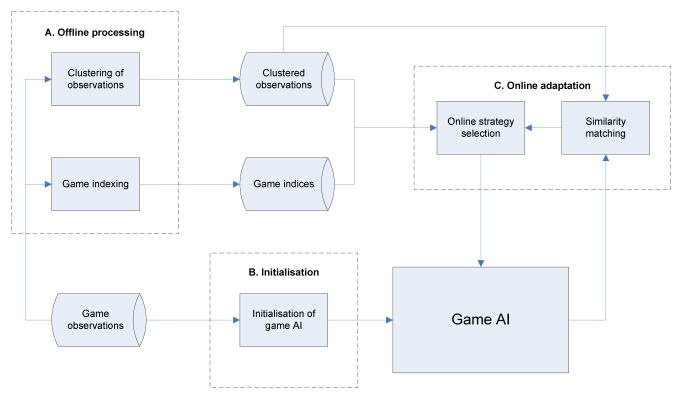
\includegraphics[width=0.5\textwidth]{ch3cbrspring}
	\caption{Proces adaptivní AI založené na CBR \cite{21cbr}}
	\label{fig:ch3cbrspring}
\end{figure}

Při inicializaci (B. Initialisation) se nastaví první strategie AI, která se ukázala nejlepší v daném scénáři. Poslední části schématu je online adaptace (C. Online adaptation), která nesmí být náročná na výpočetní výkon, jelikož se provádí v reálném čase. V určitých intervalech během hry se změní strategie hráče (Online strategy selection) na strategii, která se ukázala nejvhodnější v podobné situaci(Similarity matching).

\subsubsection{Sběr a úprava dat}

Při sběru dat pro adaptivní AI ve hře Spring získali 448 567 pozorování z celkem 975 her na třech různých herních mapách. Výsledná data zabírala 1192 MB nekomprimovaně. Spouštěli se vždy hry s dvěma protihráči. Pokaždé inicializováni různými strategiemi. V tomto kontextu se strategií míní vektor celkem 27 parametrů představující důraz na různé strategické chování na vysoké úrovni. Např. parametr aircraft\_rate ovlivňuje, jak moc často by měl hráč vytvářet vzdušné jednotky. Jakým způsobem se toho dosáhne už nesouvisí s těmito parametry. Dále je nutné popsat a uložit popis dané situace, jež se později použije pro vyhledávání podobných pozorování. Pozorování je popsáno 6 parametry. Fáze hry, síla materiálu, bezpečí velitele, ovládané území, ekonomická síla a počet vojenských jednotek.

\subsubsection{Ohodnocení her}

Každé z pozorováních se ohodnotí pomocí fitness funkce. Získané číslo určuje, kdo v dané chvíli vítězí. Fitness hodnota blížící se nule značí vyrovnané síly obou soupeřů. Vypočítá se např. z fáze hry, množství surovina a jednotek jednotlivých hráčů.

\subsubsection{Shlukování pozorování}

Shlukování je velice časově náročné, a proto se provádí offline. Cílem je nahradit více pozorováních jedním reprezentantem, který může být jedním pozorováním z původních dat, nebo pozorování vzniklé zprůměrováním podobných dat. Záleží na zvoleném algoritmu. Zde postačil dobře známý a jednoduchý algoritmus k-means.

\subsubsection{Inicializace hry}

V této fázi procesu se určí první strategie dynamické AI. Nejdříve se určí strategie, kterou využívá soupeř. Z ní se udělá abstrakce, jednotlivé hodnoty 27 proměnných se nahradí hodnotou z výčtu „málo“, „středně“, „hodně“.  Poté se naleznou v databázi pozorování s hráči podobnými soupeři a vybere se inicializační strategie, která si vedla nejlépe proti takovému hráči. Z tohoto důvodu nikdy není vybrána neefektivní strategie jako první.

\subsubsection{Online adaptace}

V průběhu hry se čas od času spustí adaptace herní strategie dle aktuálního stavu hry. Tato adaptace se skládá ze dvou částí, z porovnávání stavů a výběru strategie.

Podobnost dvou pozorování je rovna váženě sumě podobnosti šestice parametrů v jednotlivých pozorováních.

\begin{equation}
	   podobnost(poz1,poz2)=((1+f)*(0,5*u)) + mp + sc + cp + ep
\end{equation}

\begin{eqnarray*}
f &= &rozdilFazeHry(poz1,poz2) \\
u &= &rozdilPoctuJednotek(poz1,poz2) \\
mp &= &rozdilMaterialniSily(poz1,poz2) \\
sc &= &rozdilBezpecnostiVelitele(poz1,poz2) \\
cp &= &rozdilObsazenychPozic(poz1,poz2) \\
ep &= &rozdilEkonomickeSily(poz1,poz2)
\end{eqnarray*}

Samotná selekce nejvhodnější strategie se skládá ze tří kroků. Nejdříve se z databáze shluků vybere N nejbližších sousedů k aktuálnímu stavu hry dle výše uvedeného vzorce. Posléze se vybere menší podmnožina M stavů na základě herního indexu(fitness) dle zvoleného kritéria.

Zde se může projevit kombinace statické volby obtížnosti s dynamickou. Hráč si může před začátkem hry z volit jednu z pevně daných obtížností, např. lehká, normální, těžká. Vybere-li si běžnou obtížnost, bude algoritmus vybírat M stavů, jež mají fitness nejblíže k 0, která značí vyrovnané šance obou hráčů na výhru. Naopak hraje-li těžkou hru, algoritmus může vybírat pozorování s fitness odpovídající větší šance na výhru soupeřem.

Zbývá vybrat jedinou novou cílovou strategii. Z M stavů se vybere takový stav, kde strategie soupeře nejvíce odpovídá aktuální strategii soupeře v současné hře.

Na závěr nutno podotknout, že tento přístup nedává jistotu stejného chování a výsledku AI hráče jako ve vybrané hře z databáze. Při výběru se porovnávají pouze zjednodušené abstrakce stavu hry a navíc pouze s agregovanými shluky stavů. Výsledné chování hráče se může lišit od očekávaného.


\subsection{Fuzzy pravidla}

Máte-li umělou inteligenci ve své hře založenou na fuzzy pravidlech, může vás zajímat následující způsob tvorby adaptivní AI.

Základní myšlenka je jednoduchá. Mějme databázi fuzzy pravidel, kde každé z fuzzy pravidel může být aktivní, nebo vypnuté. Jestliže se hra jeví příliš těžká, vybere se některé z pravidel, a to se vypne. Naopak v případě, kdy se hra jeví příliš jednoduchá, jedno pravidlo se znovu aktivuje.

\subsubsection{Dead-end}

Autoři přístupu zvolili pro jeho testování hru jednoduchou hru Dead-end. Hráč je obklopen třemi stěnami a na čtvrté straně je východ. Jeho cílem uniknout tímto východem. Jeho snažení brání nepřátelské figury, které se naopak snaží hráče chytnout. Hráč má několik životů. Jestliže dojde ke kolizi hráče s nepřátelským duchem, jeden život ztratí. Ztratí-li všechny životy, hráč prohrává. Ve hře je navíc nastaven časový limit. Vyprší-li tento limit, hráč také prohrává. Naopak dostane-li se ven s alespoň jedním životem, vyhrává. Všechny postavičky se mohou pohybovat osmi směry.

Duchy lze rozdělit do dvou rolí. Duch nejníže vzhledem k souřadnici y tvoří předvoj a jistým způsobem ovládá ostatní duchy, obránce.

\begin{figure}
  \centering
  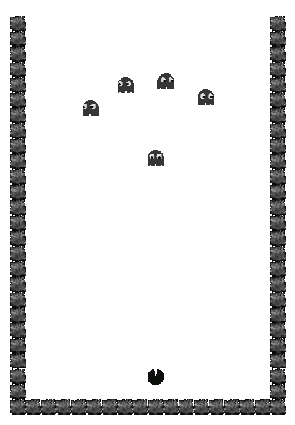
\includegraphics{ch3deadend}
	\caption{Screenshot ze hry Dead-End. \cite{25deadend} }
	\label{ch3deadend}
\end{figure}

\subsubsection{Fuzzy pravidla}

Duši se rozhodují na základě 5 vstupních fuzzy proměnných, jedné ostré proměnné a pěti výstupních proměnných.
Vstupními proměnnými pro pravidla předvoje jsou vzdálenost k hráči, vzdálenost k východu na ose y,  vzdálenost k hráči na ose x a binární proměnná, jestli duch už prošel kolem předvoje. Výstupními proměnnými jsou proměnné pro akce, které může duch provést – chytej hráče, nebo ustupuj od hráče.

Vstupní fuzzy proměnné pro obránce jsou vzdálenost k hráči, vzdálenost k předvoji, vzdálenost k nejbližšími jinému obránci na ose x a stejná binární proměnná značící, jestli byl už duch obejit.

Možné akce obránců jsou – chytej hráče, přibliž se k předvoji, oddal se od předvoje, oddal se od nejbližšího jiného obránce.
Příkladem fuzzy pravidla pro předvoj z kompletní tabulky 40 pravidel z \cite{25deadend} :
Pokud je hráč blízko předvoje a je blízko východu a hráč ještě neprošel kolem předvoje, pak chytej hráče velmi. Viz první pravidlo z následujícího obrázku Obr. \ref{fig-ch3fuzzytable}.

\begin{figure}
  \centering
  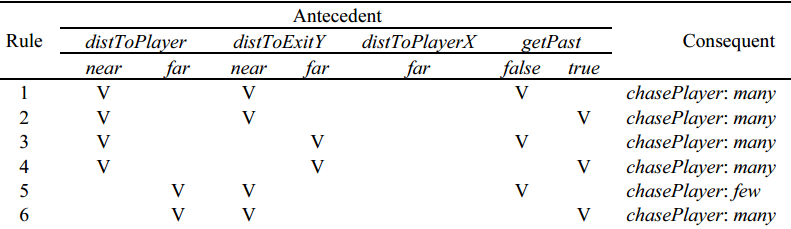
\includegraphics[width=0.75\textwidth]{ch3fuzzytable}
	\caption{Část fuzzy pravidel pro předvoj. \cite{25deadend} }
	\label{fig-ch3fuzzytable}
\end{figure}

Uvedené příklady fuzzy proměnných a pravidel by měli pro základní představu postačovat. Kompletní seznam fuzzy pravidel a detailnější popis jednotlivých proměnných včetně grafů funkce příslušnosti lze najít v již zmiňovaném zdroji \cite{25deadend}.

\subsubsection{Adaptivní změna počtu pravidel}

Jestliže se soupeř řídí všemi 40 pravidly, chová se velmi inteligentně. Hráč si na začátku hry může vybrat statickou část obtížnosti. Může ovlivnit požadovaný win-rate. Pokud tak neučiní, nastaví se win-rate na hodnotu 50\%. Každá hra trvá maximálně 20 vteřin. V případě, že hráč vyhraje a aktuální poměr vítězství/proher  je větší než cílená hodnota, hra se musí ztížit aktivováním momentálně vypnutého pravidla.

Naopak v případě, že hráč prohraje a aktuální hodnota win-rate je menší než cílená, hra je příliš těžká, zjednodušení proběhne deaktivací jednoho z pravidel.

Pokaždé, když se duch rozhodne dle jednoho z pravidel, zaznamená se to. Výsledný příspěvek se u pravidel obránců vydělí 4, jelikož jsou ve hře 4 obránci a jen jeden předvoj.

Pokud má dojít k deaktivaci pravidla, deaktivuje se pravidlo, které bylo využito nejméně krát, ale alespoň jednou. Kdyby se vyřadilo pravidlo, které se nevyužilo, hráč by nemusel vůbec změnu obtížnosti v příští hře poznat, jelikož by se mohli duchová chovat zcela stejně. Proč naopak nedeaktivovat pravidlo, které využíval soupeř nejvíce? V takovém případě by mohla být změna obtížnosti příliš drastická a mohlo by to vést k neočekávaným výsledkům.

Reaktivace pravidla je o něco složitější proces. Nejdříve se všechna pravidla rozdělí do skupin dle jejich konsekventů. Příspěvek celé skupiny pravidel je roven sumě příspěvků jednotlivých pravidel ve skupině. 

Poté se spočte suma vstupních příslušností hodnot pro každé z pravidel deaktivovaných dříve. Nakonec se zaktivuje pravidlo s největší sumou vstupních příslušností. Jestliže existují dvě pravidla se stejnou hodnotou sumy, zvolí se pravidlo jehož skupina má nejnižší příspěvek.

\subsubsection{Výsledky}

Na závěr připojuji jeden z grafů ukazující adaptivnost AI k třem různým hráčům s požadovanou hodnotou win-rate 75\% Obr. \ref{fig-ch3fuzzywinrate}. Ke srovnání na cílovou hodnotu došlo kolem 25. hry. 

\begin{figure}
  \centering
  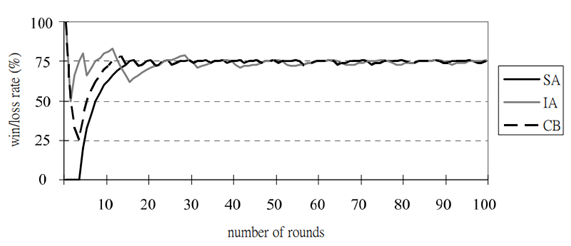
\includegraphics[width=0.75\textwidth]{ch3fuzzywinrate}
	\caption{Přibližování se k požadovanému win-rate 75\% během 100 kol proti třem různým hráčům. \cite{25deadend} }
	\label{fig-ch3fuzzywinrate}
\end{figure}

\subsection{Mravenčí feromony}

Optimalizace pomocí simulace umělých mravenčích kolonií patří mezi známé přístupy inspirované přírodou. Princip optimalizace mravenčími koloniemi je následující :


\begin{enumerate}
	\item Daný problém se vhodně modeluje jako graf skládající se z uzlů a hran mezi nimi
	\item Umělí mravenci se pohybují po hranách a zanechávají na nich feromon. Čím lépe si vedou, tím více feromonu zanechají.
	\item Mravenci se na každém uzlu rozhodují, kterou další hranou se vydají. S větší pravděpodobností zvolí hrany, na kterých je více zanechaného feromonu.
	\item Časem feromon vyprchává, je třeba obnovovat.
	\item Optimalizace končí, jestliže se ustálí cesty v grafu. 
\end{enumerate}

Tímto algoritmem se inspirovali vývojáři jedné ze serious games určené pro rehabilitaci částečně ochrnutých končetin lidí, jež utrpěli mozkovou mrtvici\cite{26poststroke}. Využití mravenčích feromonů je zde velice specifické a v tuto chvíli mě nenapadá jejich širší využití v jiné oblasti než rehabilitace částečně ochrnutých horních končetin, např. v zábavním průmyslu. Přesto je zde uvádím jako zajímavost, která stojí za zmínku.

Cílem práce bylo vytvořit hru, která budu procvičovat znovu ovládnutí pohybu ruky a zároveň bude svou obtížnost přizpůsobovat individuálním potřebám pacientů.

Výsledkem je jednoduchá hra odehrávající se na desce o rozměrech přibližně 1,5m na 1,5m rozdělená do buněk menší velikosti. Hra vždy označí některou z buněk za cílovou a pacient se jí má pokusit dosáhnout pomocí své ruky.

\subsubsection{Hráčův profil}

Schopnosti pacienta jsou zaznamenávány do tabulky Zóna schopnosti(ability zone). Zóna schopnosti je matice o velikosti m x n. Každá z buněk má přiřazeno reálné číslo reprezentující snadnost dosažení dané buňky. Cílem je vytvořit model obrazu schopností pacienta.
Tato definice pouze popisuje strukturu a zamýšlenou funkci zóny schopnosti, ale již nezmiňuje, jak takovou strukturu vytvořit. Existuje více různých cest.

Jednou z možností je uložit do každé buňky statistickou úspěšnost dosažení buňky pacientem, jestliže to dostal za úkol. Jinou možností jsou biologicky inspirovaní umělí mravenci.

Pacientova ruka představuje mravence, který se pohybuje po mřížce. Na místech, která navštíví, zanechá feromon. Feromon zanechá i na okolních buňkách, ale o něco méně. Čím více feromonu je na buňce zanecháno, tím je pro pacienta jednodušší této buňky dosáhnout, a proto je vhodnější cílit pacientovu ruku do buněk jiných.

\subsubsection{Zákon propagace}

Nově přidaná úroveň feromonu $level_s(c)$ na buňku $c$ mravencem s pozicí $s$ lze spočítat následovně.


\begin{equation}
	level_s(c)= \begin{cases}
											  A(1-\frac{dist(s, c)}{w}) & dist(s, c) \leq w \\
												0 & jinak
										 \end{cases}
\end{equation}

Ve vzorci konstanta $A$ značí nominální úroveň feromonu, jež se přidává na buňku s pozicí mravence, konstanta w značí dosah vlivu feromonu do okolních buněk. Funkce dist vrací vzdálenost mezi dvěma pozicemi předanými argumenty.

\subsubsection{Zákon vyprchávání}

Vyprchávání feromonů je též velice důležité. Zajistí zapomenutí oblastí, které hráč zasáhl pouze náhodou. Jelikož pacientovi pohyby nejsou plně kontrolovatelné, může se stát, že neúmyslně zasáhne některé buňky, které nechce.

Z tohoto důvodu chceme, aby vyprchávali více feromony, jež byly zasáhnuty náhodou. S vědomostí, které buňky zóny schopností pacient zasáhl pohybem po cestě p můžeme upravit množství feromonů na nich.

\begin{equation}
	F_{t+1} = F_t\frac{1}{vrcholyRychlosti(p)}
\end{equation}

Čím více vrcholů v grafu rychlosti na dané cestě, tím více byly pohyby trhané a tedy méně koordinované.

\subsubsection{Matice interakce}

Matice interakce je maticí m x n binárních hodnot. Jednička značí možnost vygenerovat cíl hry z odpovídající buňky, 0 naopak. V případě, že je náročnost hry odpovídající aktuálním schopnostem pacienta, matice interakce se nemění a generují se z ní nové cíle k dosažení rukou. Delší série výher značí, že hra je jednoduchá a hráč může být brzy z nuděn a nemotivován ke hře, k rehabilitaci a naopak delší série proher může způsobovat frustraci se stejným dopadem, koncem rehabilitace a možná i nechutí v ní v budoucnu pokračovat. V takovém případě se matice interakce musí přepočítat.

V obou případech se vypočítá pro každou z buněk jednoduchým vzorečkem gradient.

\begin{equation}
	grad(A_{i,j}) = \sum_{k \in \{i-1, i, i+1\}} \sum_{l \in \{j-1, j, j+1\}} A_{i, j} - A_{k, l}
\end{equation}

V případě příliš obtížné hry bude matice interakce obsahovat 1 na místech kladného gradientu, v opačném případě při příliš lehké hře bude obsahovat 1 v místech záporného gradientu. Příklad na Obr. \ref{fig-ch3feromons}.

\begin{figure}
  \centering
  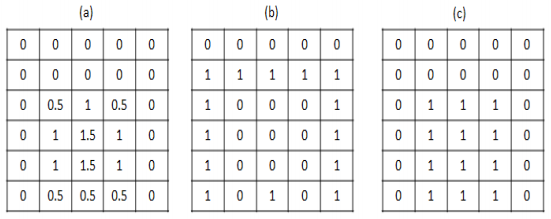
\includegraphics[width=0.75\textwidth]{ch3feromons}
	\caption{(a) Zóna schopností, (b) Interakční matice pro stížení hry, (c) Interakční matice pro zjednodušení hry \cite{26poststroke} }
	\label{fig-ch3feromons}
\end{figure}

První matice (a) obsahuje hodnoty zóny schopností po jednoduchém pohybu „zdola nahoru“ do buňky 3, 3. V matice (b) jsou jedničky na pozicích záporného gradientu dle výše uvedeného vzorce. V matici (c) jsou naopak jedničky na pozicích kladného gradientu. Z matic lze snadno vyčíst ztížení hry u matice (b) a zjednodušení u matice (c).

Jak jsem poukázal na začátku této kapitoly, jedná se spíše o zajímavost kvůli velmi specifickému užití metody mravenčích feromonů. Přesto je to inspirativní.


\section{Využitelné v teorii her}

\subsection{Částečně uspořádaná množina – Mistr}

Partially-Ordered-Set Master (POSM) \cite{22posm1} je obecně použitelným algoritmem pro dynamicky vyvažovanou obtížnost ve hrách. POSM lze využít kdykoli a v jakémkoli herním žánru. Jediným požadavkem na vývojáře je definovat konečné množství nastavení obtížnosti, pro které existuje relace „je těžší než“. Tento předpoklad není nerealistický. Většina her v současnosti obsahuje několik nastavení statické obtížnosti.

Oproti jiným přístupům DDA nevyžaduje modelaci chování hráčů. Nepředpokládá jiné znalosti o konkrétní hře. 
Základní princip algoritmu je jednoduchý. Mistr (program) inicializuje obtížnost na prostřední ze všech obtížností dle relace „je těžší než“ $\geq$. Odehraje se část hry. Posléze se určí, jestli mistr zvolil obtížnost správně dle schopností hráče, nebo jestli hra byla příliš těžká, nebo příliš jednoduchá. Na základě této informace upraví obtížnost hry správným směrem.

\subsubsection{Algoritmus POSM}

Vstupem algoritmu je částečně uspořádaná množina $(K,\geq)$ možných nastavení obtížnosti. Uspořádání je následující : $\forall i,j \in K$ píšeme $i>j$, pokud $i$ je více obtížné než $j$.
Po nastavení obtížnosti se odehraje kus hry a určí se hráčem pozorovaná obtížnost $o_t$.

\begin{itemize}
	\item $o_t=0$, jestliže obtížnost mistr zvolil správně a nemá se měnit
	\item $o_t=+1$, jestliže obtížnost byla příliš jednoduchá
	\item $o_t=-1$, jestliže obtížnost byla příliš těžká
\end{itemize}
	
Posledním vstupem algoritmu je učící konstanta $\beta\in(0,1)$. Čím blíže je konstanta hodnotě 1, tím je učení pomalejší, obtížnost je více statická.
Kroky algoritmu POSM:

\begin{algorithm}
\caption{Partially-Ordered-Set Master}
\label{posm}
\begin{algorithmic}[1]
\State $\forall k \in K : w_1(k) = 1$
\For{$i \gets 1, 2, \dots$}
	 \State $\forall k \in K : A_t(k) = \sum_{x \in K, x \geq k} w_t(x)$
	 \State $\forall k \in K : B_t(k) = \sum_{x \in K, x \leq k} w_t(x)$
	 \State $k_t = \operatorname{arg\,max}_{x \in K} \min({A_t(x), B_t(x))}$
	 \State Pozoruj reálnou obtížnost $o_t\in \{0,+1,-1\}$
	 \If{$o_t = 1$}
	   \State $\forall k \in K : w_{t+1}(k) = 
		                                        \begin{cases}
																						   \beta w_t(k) & k \leq k_t \\
																							 w_t(k) & jinak
																						\end{cases}
						 $
   \EndIf
	 \If{$o_t = -1$}
	   \State $\forall k \in K : w_{t+1}(k) = 
		                                        \begin{cases}
																						   \beta w_t(k) & k \geq k_t \\
																							 w_t(k) & jinak
																						\end{cases}
						 $
   \EndIf
\EndFor
\end{algorithmic}
\end{algorithm}

Na prvním řádku se inicializuje vektor w představující hodnoty „správnosti“ volby každé z obtížností. Na 3. řádku se uloží ke každé obtížnosti suma správnosti obtížností, které jsou těžší, nebo stejné než ona. Na 4. řádku se naopak uloží ke každé z obtížností suma správnosti obtížností, kterou jsou lehčí, nebo stejné než ona. Na pátém řádku se volí nová obtížnost dle uvedeného vzorce. Poté proběhne kus hry a algoritmus získá odpověď o reálné obtížnosti vzhledem k hráči. Na následujících řádcích se „správnosti“ jednotlivých obtížností vhodně upraví do další iterace hry.

\subsubsection{Příklad s balónky}

Algoritmus se lépe vysvětlí na příkladě.\cite{23posm2} Mějme jednoduchou hru sestřelování padajících balónků. Hráč je má sestřelit dříve než se dotknou země. Obtížností hry může být rychlost padání. Mějme předpřipraveno 10 různých rychlostí odpovídajících 10 nastavením obtížnosti.

Při inicializaci se vektor $w$ nastaví na 10 jedniček. Při prvním běhu bude vektor $A$ obsahovat $(10; 9; 8; 7; 6; 5; 4; 3; 2; 1)$ a vektor $B$ $(1; 2; 3; 4; 5; 6; 7; 8; 9; 10)$. Na 5. řádku se vybere náhodně 5. nebo 6. obtížnost, protože v obou případech :


	\[
	\max{\min{\{5, 6\}}} = \max{\min{\{6, 5\}}} = 5
\]

Po nastavení nové obtížnosti 5 může hráč hrát po předem stanovenou dobu, např. 15 vteřin. Na 6. Řádku se určí, jestli mistr dobře zvolil poslední obtížnost. V naší konkrétní hře, pokud hráč sestřelí všechny 95-100\% balónků, hra byla jednoduchá. Jestliže spadne na zem 5-15\% balónků, hra je vyvážená. Ve zbylých případech je hra příliš těžká.

V našem příkladu máme zkušeného hráče a při obtížnosti 5 sestřelil všechny balónky. Z toho vyplývá $o_t=+1$. Na řádcích 7 až 9 se provede úprava vektoru $w$. V tuto chvíli obtížnosti 1 až 5 nejsou vhodné, upraví se jejich správnost. Pro adaptivní konstantu $\beta=0,5$ bude vektor $w_2=(0,5;0,5;0,5;0,5;0,5;1,1;1;1;1)$.

Pokračujme druhou iterací. 

$A_2=(7.5;7,0;6,5;6,0;5,5;5,0;4,0;3,0;2,0;1,0)$, 

$B_2=(0,5;1,0;1,5;2,0;2,5;3,5;4,5;5,5;6,5;7,5)$

Pro přehlednost vektor minim z hodnot na odpovídajících si indexech.

$m=(0.5,1.0,1.5,2.0,2.5,3.5,4.0,3.0,2.0,1.0)$

Maximum z vektoru $m$ je hodnota 4.0, která je na 7. pozici. Hra se ztíží na 7. obtížnost.

Na uvedeném příkladě je vidět, že POSM je jednoduchým algoritmem s minimem předpokladů na znalosti konkrétní hry, a proto je použitelný pro velkou škálu užití. Vyzkoušen a testován byl např. na deskových hrách dáma a čínské šachy. \cite{23posm2}

\subsection{Dynamická úroveň}

Autoři tohoto přístupu se zaměřili na dynamické vyvažování obtížnosti v deskových hrách. \cite{24DynLev} Sami svůj algoritmus nijak nenazvali, tedy název této podkapitoly je mnou vymyšlen a google ho „nezná“. Alespoň ne ve spojitosti s tímto algoritmem.
Možnosti DDA v deskových hrách se od možností DDA v ostatních počítačových hrách výrazně liší. Ve střílečce, real-time strategii můžete obtížnost hry vyvažovat změnou pravidel hry aniž by si toho hráč všiml. Obtížnost může být dána přesností mušky botů ve hře, či množstvím zdrojů, s kterými soupeř pracuje ať už je během hry mohl, či nemohl získat.

Článek označuje jako jedinou možnost DDA v deskových hrách ovlivňovat AI soupeřů. Bohužel s tímto tvrzením nemohu souhlasit. I když se zaměříme pouze na deterministické deskové hry s úplnou informací, kterými jsou např. šachy, máme k dispozici online i offline dynamické vyvažování obtížnosti hry, které by jistě napadli většinu hráčů šachů, jelikož to již mnozí využili. Za offline DDA můžeme považovat odebrání některých herních figur před začátkem hry. K online vyvažování může patřit různé časové omezení na provedení tahu u jednotlivých hráčů. Vedoucí hráčů bude mít méně času na přemýšlení a tím se zvětší pravděpodobnost provedení chybného času a vystřídání hráčů ve vedení.

\subsubsection{Popis algoritmu}

Zpět k „dynamické úrovni“. Algoritmus má dva předpoklady k jeho využití. Vyžaduje funkci, jež umí ohodnotit všechny následující stavy ve hře. Hodnost vyjadřuje kvalitu dané situace z pohledu hráče, který je právě na tahu. Určuje šanci na výhru aktivního hráče.
Druhá funkce vrací status hry. Kdo vyhrává a jak moc. Kladné hodnoty statusu značí vedení, 0 remízu, záporné hodnoty prohrávání. Nejen znaménko statusu se bere v potaz, i hodnota je důležitá. Mělo by platit, že čím větší je hodnota statusu, tím větší šance na výhru daným hráčem.

Algoritmus je vytvořen pro dvouhráčové hry, kde jeden hráč má dynamickou úroveň. Při volbě nového tahu se řídí následujícími kroky:


\begin{enumerate}
	\item Uprav odhad soupeřovy úrovně na základě status funkce.
	\item Vygeneruj všechny možné následující stavy ze stavu aktuálního.
	\item Přiřaď hodnosti vygenerovaným stavům.
	\item Vyber následující tah jako nejvhodnější vzhledem k odhadované soupeřově úrovně.
\end{enumerate}

Pseudokód algoritmu by mohl vypadat následovně:

\begin{algorithm}
\caption{Dynamická úroveň}
\label{alg-dynlevel}
\begin{algorithmic}[1]
\State $level_1 \in \left\langle 0, 100 \right\rangle$
\For{$i \gets 1, 3, 5, \dots$}
	 \State $status_t = statusFnc(state_t)$
	 \State $level_t = \begin{cases}
											  0 & \text{pokud level} + \frac{status_t}{\alpha} < 0 \\
												100 & \text{pokud level} + \frac{status_t}{\alpha} > 100 \\
												level + \frac{status_t}{\alpha}  & \text{jinak}
										 \end{cases}
						 $
   \State $S_t = nextStates(state_t)$
	 \State $\forall s \in S_t : r_t(s) = rankFnc(s)$
	 \State $state_{t+1} = s, s \in S_t, \text{kde } r_t(s) \text{ je v } \frac{level_t}{100} \text{ pořadí seřazených s dle } r_t(s)$
	 \State $state_{t+2} = opponentTurn(state_{t+1})$
\EndFor
\end{algorithmic}
\end{algorithm}

Na prvním řádku se určí inicializační úroveň jako odhad úrovně soupeře. V článku[24] není přesně definováno, jak počáteční úroveň volit. Možností je náhodně generované číslo, případně statický výběr hráčem z několika předdefinovaných možností. Např. „lehká“ = 25, „střední“ = 50 atd.

Třetí a čtvrtý řádek slouží k novému odhadu úrovně oponenta. Figuruje zde konstanta $\alpha$, určující dynamičnost změny úrovně hráče. Konstanta je závislá na konkrétní hře. Může být volena experimentálně, nebo se může i v průběhu hry měnit např. pomocí algoritmu simulovaného žíhání.

Na řádcích 5 – 7 se vygenerují následující stavy a vybere se ten s nejvhodnější hodností dle úrovně soupeře. Příklad : existuje 20 možných tahů, které jsme ohodnotili a dle ohodnocení seřadili. Jestliže je úroveň rovna 75, zvolí se tah v $\frac{3}{4}$ seřazených tahů, tedy 5. Nejlepších tah. Po úroveň 50 se zvolí tah v polovině, tedy tah 10. ze seřazených tahů.
Na osmém řádku se počká na tah oponenta a celý cyklus se opakuje od začátku.

\subsubsection{Ohodnocovací a status funkce}

Jaký je rozdíl mezi rankFnc a statusFnc? Každá se využívá v jiné části algoritmu. Vnitřně mohou být stejné. Proč tedy autoři rozlišují funkce 2? V článku se k tomu obecně moc nevyjadřují, ale lze něco usoudit z jejich testovací hry Backgammon.
Ohodnocovací rank funkce je zde složitá a bere v úvahu mnoho parametrů popisujících stav hry. Parametry jsou např. počet kamenů již mimo hru, součet vzdáleností zbylých kamenů od konce, šance na zajetí svého kamenu soupeřem v příštím tahu, jsou-li všechny kameny alespoň ve 4. (posledním) kvadrantu hry apod.

Naopak status funkce popisuje stav hry méně složitě, více z lidského pohledu. Spočítá skóre každého hráče jako počet kamenů již mimo hru + suma vzdáleností zbylých kamenů od konce hry. Status je rozdílem těchto dvou hodnot.

\subsection{Monte-Carlo prohledávání stromu}

Autoři z Pekingské univerzity vyzkoušeli spojení Monte-Carlo Tree Search(MCTS) algoritmu s dnes populárními neuronovými sítěmi. \cite{18Pac1}\cite{19Pac2}

V článcích upozorňují na nevýhodu tradičních metod DDA, kdy se obtížnost uměle mění např. přidáváním dalších a silnějších nepřátele, ale jejich inteligence zůstává stejná. Hráč se v takovém případě může cítit podveden. V Pekingu se vydali cestou dynamického vyvažování umělé inteligence a svůj přístup aplikovali na zjednodušené verzi známé hry Pac-Man.

\subsubsection{Pravidla hry Pac-Man}

Cílem hráče hrajícího za žlutou postavu Pac-Mana je sníst všechny kuličky v bludišti a zároveň se vyhýbat nepřátelům, duchům. Pac-Man zvítězí, jestliže sní všechny kuličky, duši zvítězí, jestliže chytnou Pac-Mana. Jestliže do 55 kroků žádná z těchto událostí nenastane, hra končí remízou. Oproti původnímu Pac-Manovi jsou ve hře další úpravy.


\begin{itemize}
	\item Bludiště je zmenšeno na velikost 16x16 a neobsahuje žádné Power upy.
	\item Ve hře jsou pouze dva duši místo původních 4 a mají stejnou rychlost jako Pac-Man. Z toho vyplývá, že jeden duch nikdy nemůže sám chytit Pac-Mana, duši musí spolupracovat.
	\item Pac-Man i duši se rozhodují pouze na křižovatkách. Jejich možné akce jsou jít vpravo/vlevo/nahoru/dolů, případně u křižovatek u kraje bludiště jejich podmnožina, procházení zdí je zakázáno.
\end{itemize}

\begin{figure}
  \centering
  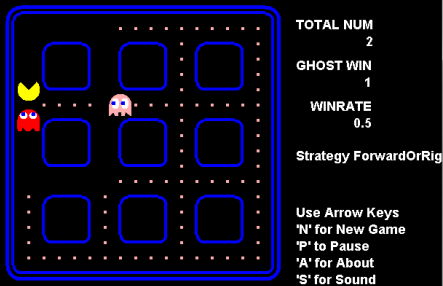
\includegraphics[width=0.5\textwidth]{ch3pacman}
	\caption{Zjednodušená verze Pac-Mana. Obrázek převzat z \cite{18Pac1}}
	\label{fig:ch3pacman}
\end{figure}

\subsubsection{Tvorba DDA pomocí MCTS}

Výkon umělé inteligence soupeřů založených na MCTS záleží na množství času, které MCTS poskytneme. Čím déle algoritmus běží, tím je pravděpodobnější inteligentnější chování duchů.

Pro účely simulace hráč Pac-Mana využíval ForwardOrRight strategii.
Pomocí opakovaných simulací s pevně daným simulačním časem získali závislost poměru vítězství (win-rate) na délce simulace. Několik získaných diskrétních hodnot proložili polynomem 4. stupně.

\begin{equation}
	y=-5,67*x^4+17,6*x^3-11,1*x^2-0,81*x+65,6
\end{equation}

V předchozí rovnici je x časem výpočtu MCTS v ms a y výsledné win-rate.
Běžný hráč chce vyhrávat přibližně v polovině případů. Vyřešením rovnice získáváme čas 105ms. Začínající hráč může upřednostnit častější vyhrávání, při win-rate 30\% (duchy) algoritmus potřebuje 28ms na výpočet.

\subsubsection{Využití neuronových sítí}
Další nevýhodou škálování AI pomocí změn simulačního času je horší využitelnost u real-time her, kde si nemůžeme dovolit věnovat stovky ms k výpočtu AI. Tento nedostatek lze odstranit využitím neuronové sítě místo MCTS.

Neuronovou síť se snažíme naučit chování odpovídající MCTS s daným simulačním časem. Při simulacích pomocí MCTS se při každém rozhodování duchů uložil stav hry, jako 23 proměnných a výsledné rozhodnutí o novém směru každého ducha.

Takto získaná data bylo použita pro učení neuronové sítě, která posléze nahradila původní algoritmus MCTS. Vstupními proměnnými byly např. pozice a směr hráče, pozice duchů a obsah sousedních dlaždic, vzdálenost mezi duchy a hráčem, čas simulace atd. Ve výstupní vrstvě bylo po 4 neuronech pro každého ducha, kde každý neuron představoval jeden zvolený směr.

Neuronové sítě odstranily časovou divergenci pro různé AI, ale naopak přinesly do systému jistou míru nepředvídatelnosti.
